
%(BEGIN_QUESTION)
% Copyright 2011, Tony R. Kuphaldt, released under the Creative Commons Attribution License (v 1.0)
% This means you may do almost anything with this work of mine, so long as you give me proper credit

{\it Reforming furnaces} are special process furnaces used to generate pure hydrogen gas from a hydrocarbon feed gas, such as methane.  Methane gas (CH$_{4}$) added to steam (H$_{2}$O) at high temperatures forms hydrogen gas (H$_{2}$) and carbon monoxide gas (CO), the latter converted into CO$_{2}$ and more hydrogen gas in subsequent reactions.  The chemical reaction is highly {\it endothermic}, meaning that it requires energy input rather than liberating energy (as what happens in an {\it exothermic} process such as combustion).  This required heat comes from a set of gas burners at the bottom of the reaction furnace:

$$\includegraphics[width=15.5cm]{i02504x01.eps}$$

The rate of hydrocarbon feed greatly ``loads'' the control of temperature inside the reaction furnace, making it more challenging to maintain setpoint temperature as the feed rate varies.  Design a solution for this temperature-stability problem using a {\it feedforward} control strategy, explaining the reasoning behind your solution.

\vskip 20pt \vbox{\hrule \hbox{\strut \vrule{} {\bf Suggestions for Socratic discussion} \vrule} \hrule}

\begin{itemize}
\item{} How would your design solution be affected if the chemical reaction inside the furnace were mildly {\it exothermic} rather than endothermic?
\item{} Predict the effects resulting from one of the transmitters in this system failing with either a {\it high} or a {\it low} signal.
\item{} Predict the effects resulting from an operator increasing the steam-to-methane ratio value ($k$).
\item{} Devise a test by which you could determine whether {\it dynamic compensation} is needed in your proposed feedforward control strategy.  Be specific, identifying how you can tell whether you will need to incorporate {\it lead} or {\it lag} into the feedforward loop to optimize its performance.
\end{itemize}

\underbar{file i02504}
%(END_QUESTION)





%(BEGIN_ANSWER)

$$\includegraphics[width=15.5cm]{i02504x02.eps}$$

%(END_ANSWER)





%(BEGIN_NOTES)


\vfil \eject

\noindent
{\bf Summary Quiz:}

Suppose the methane flow transmitter were incorrectly calibrated by an instrument technician, such that it registered less flow than there actually was going through it:

$$\includegraphics[width=15.5cm]{i02504x01.eps}$$

What effect would this calibration error have on the operation of the reforming furnace?

\begin{itemize}
\item{} The furnace temperature would rise uncontrollably
\vskip 5pt 
\item{} There would be too much methane and not enough steam
\vskip 5pt 
\item{} The furnace temperature would fall uncontrollably
\vskip 5pt 
\item{} There would be too much steam and not enough methane
\vskip 5pt 
\item{} There would be too much steam and too much methane
\vskip 5pt 
\item{} There would be too little methane and too little steam
\end{itemize}



%INDEX% Control, strategies: feedforward
%INDEX% Process: hydrogen production (reforming)
%INDEX% Process: natural gas reforming 

%(END_NOTES)


